\section{Engagement de la cible lors du CAS}

Cette section décrit les procédures standard lors du \gls{cas}. Bien que certaines opérations nécessitent des procédures spécifiques, le personnel impliqué dans le \gls{cas} doit être familier avec le format standard.

\subsection{Création du briefing par le J-TAC}
Une fois la cible désignée par le \gls{gc}, le \gls{jtac} doit effectuer les actions décrites ci-dessous.

Le processus commence à la fin et progresse à reculons, en commençant par la cible, de manière à permettre au \gls{jtac} d'établir un \gls{gp}, un \gls{cb}, ainsi que les remarques/restrictions dans un ordre logique.

Cependant, chaque étape a une influence sur les autres, et il se peut qu'il faille revenir sur un point déjà établi durant le processus. Par exemple, le \gls{sead} peut avoir une influence sur le \gls{gp}.

\begin{e1}
	
	\itemt{Rassembler les informations à propos de la cible.}{
		Il y a quatre informations dont le \gls{jtac} a absolument besoin pour planifier son attaque: l'élévation de la cible, sa description, sa position, et la position des unités alliées.
	}
	
	\begin{e2}
		
		\itemt{Élévation de la cible (ligne 4).}{
			Par défaut, l'élévation est exprimée en pieds au dessus de la mer (ft \gls{msl}).
			
			Si le \gls{jtac} choisit d'utiliser une autre unité de mesure, cela devra être clairement signifié.
		}
	
		\itemt{Description de la cible (ligne 5).}{
			La description de la cible doit être concise et précise (par ex. ``5 chars dans un champ'').
			
			Le \gls{jtac}/\gls{faca} doit éviter d'utiliser des descriptions compliquées ou des termes qui risquent de ne pas être compris par les pilotes.
			
			Cependant, la description doit rester spécifique. si le \gls{gc} veut attaquer une \gls{hvt} qui se trouve dans un building à deux étages, il devra spécifier "\gls{hvt} dans building à 2 étages", et pas seulement "building à 2 étages".
		}
		
		\itemt{Position de la cible (ligne 6).}{
			Le \gls{jtac}/\gls{faca} doit évaluer la précision minimale nécessaire pour les coordonnées de la cible pour accomplir les objectifs du \gls{gc}. Il ne faut pas perdre trop de temps à raffiner les coordonnées de la cible et prendre le risque de retarder l'action des appareils de \gls{cas} si l'approximation actuelle de la position suffit à exécuter la mission.
			
			Par exemple, un largage de bombe guidée laser depuis un émetteur au sol demandera des coordonnées beaucoup moins précises qu'une largage de \gls{jdam}.
			
			Il existe plusieurs méthodes pour déterminer la position de la cible:
		}
		
		\begin{e3}
			
			\itemt{Association du terrain et d'une carte.}{
				Le moins précis, mais rapide et efficace en fonction de la situation.
			}
			
			\itemt{\gls{lrf} couplé au \gls{gps} et/ou la boussole.}{
				Sujet à l'imprécision de la boussole, et au brouillage \gls{gps}. Si le brouillage \gls{gps} est possible, une autre méthode devra être utilisée.
			}
			
			\itemt{Logiciel de ciblage}{La méthode la plus précise.}
			
			\itemt{Coordonnées dérivées des images de reconnaissance.}{}
			
		\end{e3}
		
		\itemt{Positions alliées (ligne 8).}{
			La positions des unités alliées au sol sont données à partir de la position de la cible. La direction est donnée de manière cardinale ou sous-cardinale (N, NE, E, SE, S, SW, W, NW), et la distance est exprimée en mètres.
			
			L'observateur ou le \gls{jtac} peuvent ne pas être l'unité alliée la plus proche de la cible.
		}
		
		\itemt{Effet souhaité par le \gls{gc}.}{
			L'effet souhaité par le \gls{gc} est déterminé en parlant avec lui.
			
			Le \gls{jtac} doit offrir au \gls{gc} une estimation réaliste des possibilités en fonction des appareils disponibles, de l'armement embarqué, et de son expertise.
		}
		
	\end{e2}
	
\end{e1}

\subsection{Requête de CAS}

\begin{e1}
	\item Une fois que la position de la cible a été grossièrement estimée, le \gls{jtac} doit envoyer la demande de \gls{cas} le plus vite possible, pour prendre en compte le temps nécessaire avant l'arrivée des appareils. Il ne faut pas retarder l'envoi de la demande pour augmenter la précision des coordonnées de la cible.
	
	\important{Il ne faut jamais utiliser les coordonnées des unités alliées comme coordonnées cible dans une demande de \gls{cas}.}
\end{e1}

\subsection{Création du game plan}

Au minimum, le \gls{gp} contiendra le type de contrôle et la méthode d'attaque.

D'autres informations peuvent être intégrée au \gls{gp} ou être ajouté plus tard aux remarques du \gls{cb}: les intentions du \gls{gc}, l'effet désiré, ou l'intervalle entre les appareils dans le cas d'une attaque simultanée par plusieurs éléments \gls{cas}.

Dans le cas d'attaques séquentielles (\gls{sead}, marquage), une attention particulière devra être apportée à l'établissement de la séparation entre les appareils.

L'objectif du \gls{jtac} n'est pas de dicter aux appareils de \gls{cas} les tactiques à employer, mais de fournir un plan qui correspond aux intentions du \gls{gc}.

\begin{e1}
	
	\itemt{Déterminer l'effet désiré.}{
		La première étape consiste à déterminer l'effet désiré et la manière de créer cet effet.
		
		Les facteurs à prendre en compte sont:
	}
	
	\remark{
		\begin{e2}[2em]
			\item Composition de la cible (blindage).
			\item Répartition de la cible (centré sur un point ou dispersé).
			\item Position (dégagée ou protégée).
			\item Dégâts collatéraux potentiels.
			\item Proximité des unités alliées.
		\end{e2}
	}
	
	Il faudra aussi prendre en compte le type d'appareil \gls{cas}, leur emport probable, leurs systèmes de visée et de guidage, la façon dont l'armement peut être tiré, la menace dans et aux alentours de la zone,  et le temps nécessaire au déploiement de l'armement.
	
	Le \ja{} doit avoir une connaissance minimale de l'effet des armements, et estimer les risques. Si ces risques sont élevés, une coordination avec le \gls{gc} peut s'avérer nécessaire.
	
	Les pilotes peuvent conseiller le \ja{} dans son choix de l'armement et de la méthode de tir.
	
	\itemt{Choisir le type de \gls{tac}.}{
		Le type de \gls{tac} dépend de l'armement employé, de la meilleur manière de réduire les risques, de la vitesse de l'engagement et de la capacité du \gls{jtac} à voir la cible et/ou l'appareil qui attaque.
	}
	
	\itemt{Choisir la méthode d'attaque (\gls{boc} ou \gls{bot}).}{
		La méthode d'attaque est choisie de manière à permettre l'attaque la plus rapide possible, en fonction du type de cible, de la façon dont sera acquise la cible, et de la situation.
	}
	
	\itemt{Planifier l'intervalle entre les appareils.}{
		Le \gls{jtac} peut demander un intervalle spécifique entre les attaques, en fonction de la cible, des menaces, des activités alliées, de la déconfliction artillerie/\gls{sead}/laser, de l'armement utilisé, des restrictions, de la météo, etc.
		
		Les pilotes se doivent d'adapter leur tactiques pour respecter le timing et les intervalles imposés.
	}
	
	\begin{e2}
		
		\itemt{Attaque simultanée.}{
			Tous les appareils délivreront leur armement de manière à créer un effet simultané.
			
			Cette méthode minimise l'exposition des appareils aux menaces et offre à l'ennemi un temps de réaction très court.
			
			C'est la méthode optimale pour engager des cibles multiples, tout particulièrement des unités mobiles qui pourraient fuir après la première attaque.
			
			Le principal désavantage de cette méthode est l'impossibilité de corriger ou d'annuler le tir entre les impacts et la diminution du support mutuel entre les appareils qui attaquent.
			
			\important{Un attaque simultanée nécessite que les appareils utilisent des codes laser différents.}
		}
		
		\itemt{Attaque séquentielle.}{
			Les appareils attaquent un à la fois, avec un intervalle spécifique entre les attaques, basé sur le temps nécessaire à l'acquisition de l'appareil précédent, la durée de vol de l'arme employée, le temps nécessaire au dégagement visuel de la zone attaquée (fumée, fragments, etc.), et le temps nécessaire à évaluer l'efficacité de la frappe précédente et le besoin d'une nouvelle frappe.
			
			Quelques guides pour les attaques séquentielles:
		}
		\begin{e3}
			\item 30 secondes pour un contrôle de \gls{typeone} avec des bombes lisses.
			\item 1 minute pour des \gls{lgb} délivrées à altitude moyenne.
			\item Plus de deux minutes pour décider de la ré-attaque lors de l'emploi de \gls{pgm} à haute ou moyenne altitude.
		\end{e3}
		
		\itemt{Développer un plan d'utilisation des senseurs.}{
			Le \ja{} doit prendre en compte le temps nécessaire à la mise en oeuvre et à l'utilisation des différents senseurs embarqués.
			
			\todo[inline]{Lien vers la section ISR du chapitre 3}
		}
	\end{e2}
\end{e1}

\subsection{Détermination du type de marque et de l'aide à la corrélation}

\begin{e1}
	
	\itemt{\glsfull{boc}.}{}
	
	\begin{e2}
		\item Pas de marque nécessaire (ligne 7: "No mark").
		
		\item Si le \gls{tac} est utilisé avec des \gls{lgw}, le call-sign de l'unité qui fournit le \gls{tac} et le code laser seront fournis.
		
		Exemple de ligne 7: "Blackjack laser, code 1688".
	\end{e2}
	
	\itemt{\gls{bot}.}{
		La marque dépendra de l'appareil qui attaque.
	}
	
	\itemt{\gls{bot} et contribution d'une tierce partie.}{}
	
	\begin{e2}
		
		\itemt{Tierce partie.}{
			Suite l'expansion des technologies déployées sur le champ de bataille, le \gls{jtac} peut décider de recourir à une tierce partie (unité \gls{recce}, sniper, appareils équipés d'un émetteur laser, etc.) pour aider à l'obtention des coordonnées ou de la position de la cible, à l'attaque terminale ou à l'établissement du \gls{bda}.
			
			De ce fait, la corrélation entre les pilotes ou le \ja{} et ces parties tierces sera également nécessaire.
		}
		
		\item{Considérations.}{}
		
		\begin{e3}
			\item Les pilotes utilisent généralement une combinaison de senseurs et leurs yeux pour acquérir les marques et les cibles.
			
			Par exemple, un pilote de \gls{fw} peut utiliser un \gls{lst} pour traquer l'origine du ciblage laser du \gls{jtac} et ainsi obtenir sa position.
			
			Les \glspl{jtac} doivent être familiers avec les capacités des senseurs et utiliser des marques qui utilisent ces capacités.
			
			\item Le \gls{jtac} doit toujours avoir en réserve un plan de marquage alternatif.
		\end{e3}
		
		\itemt{Types de marque et \gls{tgo}.}{}
		
		\begin{e3}
			
			\itemt{Marquage laser.}{
				La marque laser utilise un \gls{ltd} pour fournir l'énergie laser au \gls{lst} de l'appareil.
				
				Le \gls{ltd} peut se trouver au sol ou embarqué dans un autre appareil.
			}
			
			\begin{e4}
				\item Avantages:
				\begin{e5}
					\item Excellente corrélation de la position de la cible si la géométrie correcte est utilisée.
					\item Peut être utilisé de jour comme de nuit.
				\end{e5}
				\item Désavantages:
				\begin{e5}
						\item Nécessite un \gls{ltd} et un \gls{lst}.
						\item Demande de la coordination géométrique pour le \gls{lst} ne traque pas le \gls{ltd} (l'origine du pointage).
						\item Le marquage laser depuis le sol est souvent difficile, particulièrement lorsque l'unité qui effectue le pointage est sous le feu ennemi.
						\item Un premier passage d'acquisition de la marque est parfois nécessaire.
				\end{e5}
				\important{Lors du marquage laser depuis le sol, un \gls{fah} sera obligatoirement donné, de manière à renforcer l'établissement de la géométrie correcte.}
			\end{e4}
			
			\itemt{Marquage infrarouge (\acrshort{sparkle}).}{
				Les pilotes utiliseront leur \gls{nvg} pour acquérir la cible.
			}

			\makebox[\textwidth]{\centering 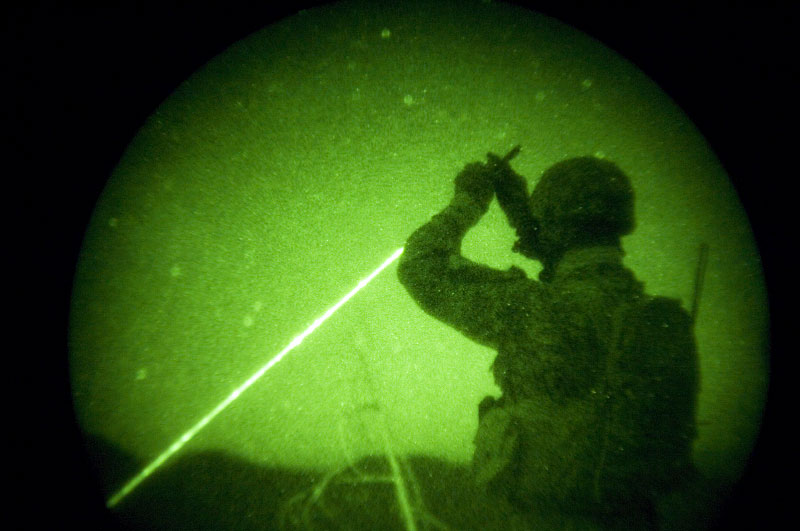
\includegraphics[width=0.5\textwidth]{niceties/ir}}

			\important{Les pilotes doivent appeler "VISUEL SPARKLE", "TALLY SPARKLE" ou "CONTACT SPARKLE" quand un marquage infrarouge est utilisé à partir du sol.}
			\begin{e4}
				\item Avantages:
				\begin{e5}
					\item Rapide.
					\item Le \gls{jtac} a la confirmation visuelle que le pilote a bien acquis la cible correcte.
				\end{e5}
				\item Désavantages:
				\begin{e5}
					\item De nuit seulement.
					\item Requiert de la coordination géométrique pour s'assurer que le pilote a bien acquis la fin du faisceau infrarouge et non pas sa source.
					\item S'il y a plusieurs pointeurs \gls{ir} près d'une même cible, il devient difficile pour le \gls{jtac} de déterminer si le pointeur se trouve bien sur la cible à cause du phénomène de ``diffusion'' dans les \gls{nvg}.
					\item Si l'ennemi dispose également de \gls{nvg}, l'utilisation d'\gls{ir} expose l'opérateur et supprime le facteur de surprise.
				\end{e5}
			\end{e4}
			
			\itemt{Walk-on infrarouge (\acrshort{sparkle}).}{
				Diriger, par une discussion entre le \gls{jtac} et le pilote, le pointeur infrarouge de l'appareil sur la cible.
			}
			
			\begin{e4}
				\item Avantages:
				\begin{e5}
					\item Ne nécessite pas que l'opérateur au sol révèle sa position aux unités ennemies équipées \gls{ir}.
					\item Le \gls{jtac} a la confirmation visuelle que le pilote a bien acquis la cible correcte.
				\end{e5}
				\item Désavantages:
				\begin{e5}
					\item De nuit seulement.
					\item Les ennemis équipés de \gls{nvg} sauront qu'ils sont pris pour cible.
					\item Du fait de la différence de perspective, il peut être très difficile de diriger efficacement le pointeur \gls{ir}.
				\end{e5}
			\end{e4}
			
			\itemt{Marquage à partir d'un \gls{trp}.}{}
			
			\begin{e4}
				\item Avantages:
				\begin{e5}
					\item Prêt rapidement si le pilote connaît le \gls{trp}.
					\item De jour comme de nuit.
					\item Offre un point de référence commun pour le talk-on.
				\end{e5}
				\item Désavantages:
				\begin{e5}
					\item Nécessite le pilote connaisse le \gls{trp}.
				\end{e5}
			\end{e4}
			
			\itemt{Marquage \gls{idf} (fumigène).}{}
			
			\begin{e4}
				\item Avantages:
				\begin{e5}
					\item De jour comme de nuit (obus phosphorescents ou lumineux).
					\item Le \gls{jtac} ne doit pas dévoiler sa position.
					\item Offre un point de référence commun pour le talk-on.
				\end{e5}
				\item Désavantages:
				\begin{e5}
					\item Prend du temps à coordonner.
					\item Le manque de précision implique souvent une correction supplémentaire à partir de la marque.
					\item Le tire indirect implique une déconfliction supplémentaire.
					\item Le \gls{fov} des senseurs peut être un problème si la marque se trouve en dehors.
					\item L'illumination de nuit sature les \gls{nvg}.
					\item Sacrifie l'effet de surprise.
				\end{e5}
			\end{e4}
			
			\itemt{Marquage par feu direct.}{
				Le marquage par feu direct utilise un tir direct (munitions traçantes ou grandes fumigènes) pour diriger l'attention du pilote sur les impacts et révéler ainsi la cible.
			}
			
			\begin{e4}
				\item Avantages:
				\begin{e5}
					\item Facilement accessible:
				\end{e5}
				\item Désavantages:
				\begin{e5}
					\item Risque de dommages collatéraux.
					\item Difficulté pour les \gls{rw} d'acquérir visuellement la marque de jour.
					\item Difficulté pour les \gls{fw} d'acquérir visuellement la marque de jour comme de nuit.
					\item Le \gls{fov} des senseurs peut être un problème si la marque se trouve en dehors.
					\item L'illumination de nuit sature les \glspl{nvg}.
					\item Sacrifie l'effet de surprise.
				\end{e5}
			\end{e4}
			
			\itemt{Considérations pour le marquage de nuit:}{}
			\begin{e4}
				\item La visibilité limitée et le manque de perspective rend la corrélation de nuit difficile.
				\item L'illumination du champ de bataille doit être planifiée de manière à ne pas saturer les \glspl{nvg}.
			\end{e4}
			
			\itemt{Marques d'opportunité.}{
			N'importe quoi sur le champ de bataille peut servir de marque; un bâtiment en feu, le trafic routier, etc.
			}
			
		\end{e3}
	\end{e2}
\end{e1}
	
\subsection{Détermination la géométrie d'attaque}

Les \glspl{jtac} doivent prendre de nombreux facteurs en compte lors de l'établissement de la géométrie d'attaque:

\begin{e1}
	\itemt{\glsfull{fah}}{
		Voir Chapitre 3, \smallref{tofah} pour plus d'informations sur le \gls{fah}.
	}
	
	\begin{e2}
		\item Le \ja{} doit éviter d'établir un \gls{fah} qui fait passer l'appareil en attaque au-dessus d'une position occupée par un allié (sol,\gls{bp}, \gls{ha}, \ldots{}).
		
		\item Le \ja{} doit prendre en compte le fait que certains appareils ont la capacité de tirer à gauche ou à droite de leur axe longitudinal (canon mobile, armes intelligentes, \ldots{}).
		
		\item le \ja{} doit prendre en compte la possibilité de ricochets ou de rebonds, et planifier le \gls{fah} parallèle à la \Gls{flot} si possible.
		
	\end{e2}
	
	\item La déconfliction latérale ou verticale avec les autres appuis-feu peut s'avérer nécessaire si la déconfliction horaire n'a pas été possible.
	
	\item Géométrie laser.
	
	\item Orientation/disposition de la cible:
	
	\begin{e2}
		
		\item Pour les cible alignées, le \gls{fah} doit de préférence être aligné avec les cibles.
		
		\item Pour les cibles en mouvement, le \gls{fah} doit de préférence être aligné sur l'axe de progression de la cible.
		
		\item Obstacles:
		
		\begin{e3}
			
			\item Canyons urbains: le \gls{fah} doit de préférence être aligné sur les canyons urbains.
			
			\item Terrain: certains éléments du terrain (montagnes par exemple) peuvent grandement influencer le choix du \gls{fah}.
			
		\end{e3}
		
		\item Météo:
		
		\begin{e3}
			
			\item Vent: un vent de travers de plus de 30kts peut affecter la précision des armes guidées.
			
			Les priorités pour le \gls{fah} sont vent arrière, vent debout, et finalement vent de travers.
			
			\item Position/angle du soleil ou de la lune:
			
			\begin{e4}
				
				\item Il faut éviter de faire attaquer les appareils avec le soleil ou la lune de face.
				
				\item Attaquer le soleil dans le dos fournit une protection supplémentaire contre les \glspl{manpad}.
				
			\end{e4}
			
			\item Nuages:
			
			\begin{e4}
				
				\item Peuvent empêcher le \gls{jtac} de voir les appareils qui attaquent.
				
				\item Peuvent empêcher les appareils qui attaquent de trouver la cible.
				
			\end{e4}
			
		\end{e3}
		
		\item Autres restrictions \glspl{acm}/\glspl{fscm} pré-planifiées.
		
		\item Le \ja{} doit déterminer l'\gls{ip}/\gls{bp} et le plan d'egress de manière cohérente avec la géométrie d'attaque (lignes 1, 2, 3, 9).
		
		Le \ja{} fait son possible pour utiliser des points d'ingress/egress qui n'imposent pas aux appareils de larges virages pour respecter le \gls{fah}.
		
	\end{e2}
	
	\itemt{Nécessités \gls{sead}/Plan \gls{sead}}
	
	\begin{e2}
		
		\item S'il n'est pas possible d'éviter la menaces sol-air, un plan \gls{sead} devra être établi.
		
		\item Le \gls{sead} et le \gls{cas} peuvent se retrouver à engager le même groupe cible; il faut alors faire attention à ce qu'il ne s'empêche pas l'un l'autre de travailler.
		
		\item La menace peut également être réduite au moyen de:
		
		\begin{e3}
			
			\item Séparation latéral: employer des armes à longue portée.
			
			\item Séparation verticale: rester au dessus de l'enveloppe de tir de la menace.
			
			\item Masquage terrain:
			
			\begin{e4}
				
				\item Tir pop-up.
				
				\todo[inline]{For examples of SEAD integration, see Appendix E, “Examples of Close Air Support Missions,” Examples 1 and 7.}
				
			\end{e4}
			
		\end{e3}
		
	\end{e2}
	
\end{e1}

\subsection{Template d'exécution du CAS}

Par sa nature même, l'exécution du \gls{cas} diffère lors de chaque mission.

Les grandes lignes restent cependant toujours les mêmes.

La template suivante fournit un cadre de travail pour le \ja{} et les pilotes.

\remark{Le déroulement présenté ici commence après le décollage, et se termine lorsque la patrouille de \acrshort{cas} est sur le retour.}

\subsubsection{Routing}

Directement après le check-in, le \ja{} doit fournir au pilote une liste des autres \glspl{aos}, leur call-sign, l'altitude à laquelle ils opèrent, et leur fréquence de travail, ce dès que possible.

Le \ja{} doit communiquer au pilote l'espace aérien disponible et la position de l'\gls{ip}/\gls{ha} pour l'attaque.

Lors du check-in initial, le \ja{} donnera, dans l'ordre:

\begin{e1}
	
	\begin{minipage}{\linewidth}
		\itemt{Instructions de transit/Instructions d'attente}{
			Lors du contact initial, le contrôleur donnera au moins une instruction du type ``Maintenez'', de manière à établir le contrôle:
		}
		
		\begin{lstlisting}[caption=Routing: maintenez, label=routingmaintain]
	REDWOLF, maintenez Chevy 14.
		\end{lstlisting}
	\end{minipage}
	
	\begin{e2}
		
		\begin{minipage}{\linewidth}
			\item S'il n'est pas certain de l'altitude actuelle de l'appareil, le \ja{} devra la demander:
			
			\begin{lstlisting}[caption=Routing: demande de position, label=routingask1]
			REDWOLF, donnez position et altitude.
			\end{lstlisting}
		\end{minipage}
		
		\begin{minipage}{\linewidth}
			\item Si un \gls{kh} non-briefé est utilisé, le \ja{} doit donner le point Echo au pilote avant de donner les informations de transit:
			
			\begin{lstlisting}[caption=Routing: keyhole, label=routinkh]
	REDWOLF, Keyhole effectif, point Echo 43 52.1N 042 43.8E, allez Alpha 10km, 500m, rappelez "é"tabli.
			\end{lstlisting}
		\end{minipage}
		
		
	\end{e2}
	
	\begin{minipage}{\linewidth}
		\item S'il n'y a pas d'autre \gls{aos}, cela devra être dit:
		
		\begin{lstlisting}[caption=Routing: pas d'autre AOS, label=routingnoaos]
	REDWOLF, allez sur Chevy, maintenez 500m, vous "ê"tes seul en station.
		\end{lstlisting}
	\end{minipage}
	
	\item Autres informations pour la sécurité du vol:
	
	\begin{e2}
		
		
		
		\begin{minipage}{\linewidth}
			\item Menaces immédiates:
			
			\begin{lstlisting}[caption=Routing: menace immédiate, label=routingthreat]
	REDWOLF, allez de Emily "à" Adder restez en dessous de 100m, ZSU23 "à" proximit"é"de l'usine 34, vous "ê"tes seul en station.
			\end{lstlisting}
		\end{minipage}
		
		\item Fait marquant à propos de la météo ou du terrain.
		
	\end{e2}
	
	\item Pour maintenir sa \gls{sa} quant à la position des différents appareils, le \ja{} pourra demander des mises à jours de statut durant la phase de routing.
	
	\begin{minipage}{\linewidth}
		\item Exemples d'appels de routing et sécurité:
		
		\begin{lstlisting}[caption=Routing: exemple 1, label=routingex1]
	REDWOLF, allez sur Frog, maintenez 300m, sur Frog descendez et maintenez 100m, rappelez "é"tabli, standby pour le check-in, vous "ê"tes seul en station.
		\end{lstlisting}
		
		\begin{lstlisting}[caption=Routing: exemple 2, label=routingex2]
	REDWOLF, allez sur la HA Betty, restez en dessous de 1000m, artillerie alli"é"e 12 tire, direction 340, vous "ê"tes seul en station.
		\end{lstlisting}
	\end{minipage}

\end{e1}

\subsubsection{Check-in}

La procédure de check-in est essentielle pour le passage des informations entre les pilotes et les agences de contrôle.

Les agences de contrôle doivent tenir les pilotes à jour des évolutions de la situation durant le transit vers la zone de combat.

C'est pourquoi il est important que le\ja{} tiennent les agences de contrôle informées de la situation, de façon à ce que les appareils arrivent sur zone disposent déjà des dernières informations.

\begin{e1}
	
	\begin{minipage}{\linewidth}
		\item Le \ja{} choisit le moment auquel les appareils \gls{cas} envoient leur check-in:
		
		\begin{lstlisting}[caption=Check-in: envoi, label=checkinsend]
	REDWOLF, envoyez votre check-in.
		\end{lstlisting}
	\end{minipage}
	
	\item Il peut y avoir plusieurs raisons pour retarder ou abréger un check-in.
	
	Le \ja{} peut ne pas être prêt, ou en attente de contact par un autre appareil.
	
	Si l'appareil est prévu dans l'\gls{ato}, et que le \ja{} a une copie de cet \gls{ato}, le check-in peut se résumer à ``As fragged'' (comme prévu) ou ``As fragged, with exception: \ldots{}'' (comme prévu, à l'exception de: \ldots{}), pour gagner du temps sur la suite des transmissions.
	
	Si l'appareil doit passer par plusieurs contrôleurs, il peut être judicieux de réserver le check-in complet au \ja{} avec lequel l'attaque finale sera effectuée.
	
	\begin{minipage}{\linewidth}
	\begin{lstlisting}[caption=Check-in: standby, label=checkinstandby]
	REDWOLF, standby check-in, attaque en cours.
	\end{lstlisting}
	\end{minipage}
	
	\begin{minipage}{\linewidth}
	\begin{lstlisting}[caption=Check-in: autre contrôleur, label=checkinothercontrol]
	REDWOLF, PIRATE prendra votre check-in, contactez le sur Isabelle.
	\end{lstlisting}
	\end{minipage}
	
	\item Authentification: si les communications ne sont pas sécurisées, une authentification devra être effectuée. Cfr. \cruderef{dryad}.
	
	\item En fonction de la situation, le \ja{} peut demander à n'avoir que certaines parties du check-in.
	
	\begin{minipage}{\linewidth}
		\item Format du check-in:
		\begin{figure}[H]
			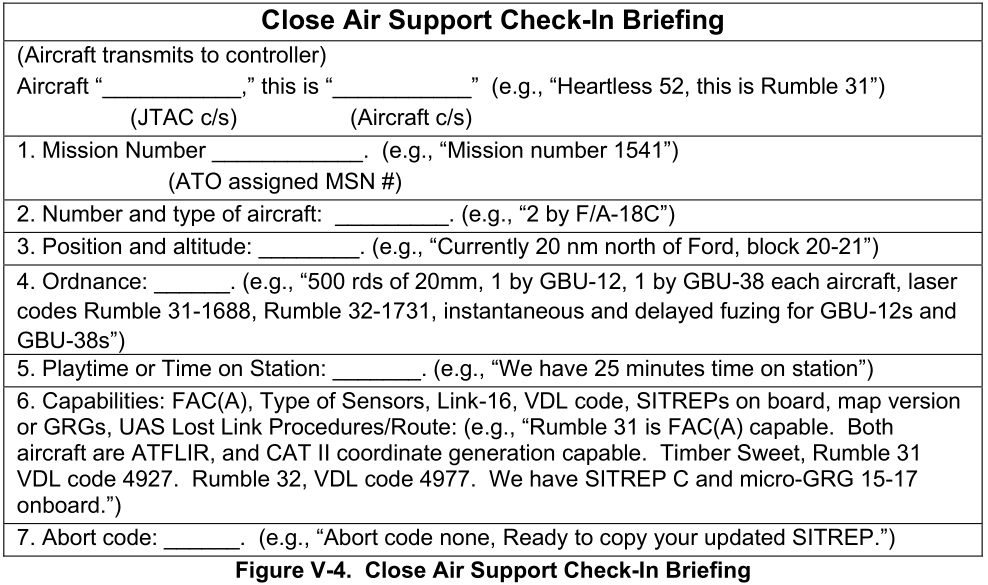
\includegraphics[width=\textwidth]{checkin.png}
			\caption{Format check-in.}
			\label{fig:checkin}
		\end{figure}	
	\end{minipage}
	
	\begin{minipage}{\linewidth}
		\itemt{Format du check-in:}{}
		\begin{lstlisting}[caption=Check-in: partiel, label=checkinpart]
	REDWOLF, pas de check-in complet, donnez armement et play-time.
		\end{lstlisting}
	\end{minipage}
	
	\begin{e2}
		\item Numéro de mission.
		\item Nombre et type d'appareils.
		\item Position et altitude.
		\item Armement:
		\begin{e3}
			\item Code laser pour les \glspl{lgb}.
			\item Type.
			\item Configuration de mise à feu (instantanée, retardée, au dessus du sol).
		\end{e3}
		\item Play-time/\gls{tos}.
		\item Capacités:
		\begin{e3}
			\item Dernier SITREP/AO Update reçu.
			\item Version du \gls{grg} à bord
			\item Capacités \gls{faca}.
			\item Capacité des senseurs.
		\end{e3}
		\item Code Abort:
		\begin{e3}
			\item Sur un réseau sécurisé, un code Abort n'est pas nécessaire, l'appel ``ABORT, ABORT, ABORT'' suffira.
			\item Sur un réseau non-sécurisé, un mot code sera établi selon les \gls{spins}/\glspl{sop} en place (ex: RAMROD, \hyperref[dryad]{DRYAD}).
		\end{e3}
		\item Si le \ja{} n'est pas familier avec le type d'appareil, il devra maintenant poser les questions en clair de manière à éviter de donner plus tard des instructions impossibles à suivre.
	\end{e2}
	
	\itemt{Situation Update}{}
	
	\begin{e2}
		\item La Situation Update est un outil utilisé pour augmenter la \gls{sa} de tous.
		
		La Situation Update peut inclure:
		
		\begin{e3}
			
			\item Activités ennemies.
			\item Activités des menaces.
			\item Situation alliée.
			\item Remarques.
			\item Météo.
			\item Dangers.
			
		\end{e3}
		
		\item Exemples d'AO Update:
		
		\efig{aoupdate1}{AO Update: exemple 1.}
		
		\efig{aoupdate2}{AO Update: exemple 2.}
		
		\begin{e3}
			\item La longueur de l'AO Update doit être adaptée en fonction du temps disponible.
			
			L'objectif de l'AO Update est de donner au pilote une \gls{sa} suffisante pour remplir sa mission.
			
			Les AO Update qui sont lues trop vite, sont trop longues, ou donnent des informations inutiles, font perdre du temps et contribuent à réduire la \gls{sa} de tous.
			
			Une AO Update particulièrement longue doit être fragmentée en plusieurs transmissions.
			
			\item Lorsque c'est possible, l'AO Update doit être transmises aux agences de contrôle, pour qu'elles puissent en informer les appareils en transit.
			
			Aussi, la transmission de l'AO Update peut être déléguée au \gls{faca}/\gls{taca}, pour permettre au \gls{jtac} de se concentrer sur le \gls{tac}.
			
			\itemt{Codage des AO Updates}{
				Les AO Updates reçoivent un codes alphanumérique, qui est transmis en même temps que l'AO Update.
				
				Cela permet au \ja{} de savoir si un pilote dispose de la dernière AO Update.
			}
			
			\begin{minipage}{\linewidth}
				\itemt{Format du check-in:}{}
				\begin{lstlisting}[caption=AO Update: code, label=aoupdatecode]
	REDWOLF ici MAGIC, avec AO Update Charlie, rappellez pr"ê"t "à" copier.
	...
	PIRATE ici REDWOLF, pour le check-in.
	...
	PIRATE ici REDWOLF, ..., AO Update Bravo "à" bord.
				\end{lstlisting}
			\end{minipage}
			
		\end{e3}
		
	\end{e2}
	
\end{e1}

\subsubsection{Game-plan}

Le Game-plan est une méthode concise d'informer les pilotes des intentions du \ja{}.

\efig{gameplan}{Game-plan: exemple.}

\begin{e1}
	\item S'il reste des questions quant aux capacités de l'appareil, elles doivent être élucidées.
	
	\begin{minipage}{\linewidth}
		\item Le Game-plan est utilisé pour les attaques simples ou multiples.
		
		Si plusieurs appareils sont prévus pour l'attaque, il faut essayer de ne transmettre le Game-plan qu'une seule fois:
		\begin{lstlisting}[caption=AO Update: code, label=aoupdatecode]
	REDWOLF et BOURDON, dans l'ordre, rappellez pr"ê"t "à" copier le Game-plan.
		\end{lstlisting}
	\end{minipage}
	
	\item Pour les attaques multiples, le termes ``dans l'ordre'' (in order) est utilisé pour indiquer l'ordre dans lequel les appareils doivent répondre au \ja{}.
	
	Pour les attaques multiples, les éléments suivants doivent être renseignés:
	
	\begin{e2}
		
		\item Type d'attaque coordonnée:
		
		\begin{e3}
			
			\item Type d'attaque: combinée ou par secteurs
			
			\item Timing: simultanée, séquentielle, ou aléatoire.
			
		\end{e3}
		
		\item Conduite de l'attaque:
		
		\begin{e3}
			
			\item Attaque combinée: méthode de séparation (visuelle, temporelle, altitude).
			
			\begin{minipage}{\linewidth}
				
				\item Attaque par secteurs: secteurs respectifs pour chaque élément.
				
				Par exemple:
				
				\begin{lstlisting}[caption=Game-plan: attaque par secteurs, label=gameplansector]
	REDWOLF et BOURDON, ce sera une attaque simultan"é"e par secteur, REDWOLF "à" l'est, BOURDON "à" l'ouest. REDWOLF, rappellez pr"ê"t pour le Game-plan.
				\end{lstlisting}
			\end{minipage}
			
		\end{e3}
		\begin{minipage}{\linewidth}
		\item Le \ja{} donnera au premier élément le Game-plan complet, le CAS-brief, les remarques et les restrictions avant de donner le Game-plan aux second élément.
		
		Le second élément doit écouter cette transmission: si certains éléments sont communs, le \ja{} donnera au second élément les différence uniquement.
		
		Par exemple:
		
		\begin{lstlisting}[caption=Game-plan: game-plan commun, label=gameplancommon]
	REDWOLF et BOURDON, ce sera une attaque s"é"quentielle combin"é"e, REDWOLF attaque en premier, suivi par BOURDON 2 minutes apr"è"s impact. REDWOLF, rappellez pr"ê"t pour le Game-plan.
		\end{lstlisting}
		\end{minipage}
		
		\item Pendant le briefing d'attaques multiples, le \ja{} peut appeler ``standby read-backs'', pour demander au pilote de ne pas effectuer le read-back immédiatement après la transmission des informations.
		
		Le \ja{} demandera un read-back séquentiel de tous les pilotes une fois le briefing terminé.
		
		\item Marque laser par une tierce partie: lorsqu'une tierce partie assure la marque laser, son call-sign et le code laser utilisé sera donné en Ligne 7.
		
		
	\end{e2}
	
\end{e1}

\subsubsection{CAS-brief}

Le \ja{} utilisera un format standard pour transmettre le CAS-brief, d'application pour les \glspl{fw} comme pour les \glspl{rw}.

Ce format est appelé \glsfull{9l}.

La \gls{9l} est transmise d'une traite.

Les en-têtes des lignes ne sont pas transmis.

Le format est le suivant:

\efig{9line}{Format 9-Line}

\remark{L'\citetitle{atp63} stipule qu'un \gls{faca} OTAN passera l'intitulé des lignes, pour chaque ligne.}

\begin{minipage}{\linewidth}
	Si les lignes 1-3 sont abrégée, la \gls{9l} commencera par le mot ``Élévation''.
	\begin{lstlisting}[caption=9-Line: lignes 1-3 abbrégée, label=9labbr]
	Depuis la verticale. Elevation, 324... .
	\end{lstlisting}
\end{minipage}
	


\begin{minipage}{\linewidth}	
	Le \ja{} peut avertir le pilote avant la transmission de la \gls{9l}:	
	\begin{lstlisting}[caption=9-Line: avertissement, label=9loavert]
	REDWOLF, rappellez pr"ê"t "à" copier la 9-Line.
	\end{lstlisting}
\end{minipage}
	
\begin{e1}
	\itemt{Ligne 1: \glsfull{ip} ou \glsfull{bp}}{
		L'\gls{ip} est le point de départ de l'attaque.
		
		Pour les \glspl{rw}, la \gls{bp} est l'endroit où commencent les attaques.
		
		La ligne 1 contient:
	}
	
	\begin{e2}
		
		\item Nom de \gls{ip}/\gls{bp}.
		
		\item Position de la \gls{ip}/\gls{bp} ``jetable'' (par exemple \gls{kh}).
		
	\end{e2}
	
	\itemt{Ligne 2: Cap et offset}{
		Le cap est donné en degrés magnétique de l'\gls{ip} vers la cible, ou depuis le centre de la \gls{bp} vers la cible.
		
		Le \ja{} peut donner un offset s'il le souhaite.
		
		\important{Le cap est donné en 3 chiffres.}
	}
	
	\itemt{Ligne 3 - Distance}{
		Pour les \glspl{fw}, la distance est donnée en miles nautiques, au dixième de mile nautique, entre l'\gls{ip} et la cible.
		
		Pour les \glspl{rw}, la distance est donnée en mètres, entre le centre de la \gls{bp} et la cible.
	}
	
	\itemt{Ligne 4 - Élévation de la cible}{
		L'élévation est données en \gls{ft} \gls{msl}.
	}
	
	\begin{e2}
		
		\item L'élévation est lue comme une séquence de chiffres.
		
		Il est recommandé d'inclure le mot ``pieds'' à la fin pour marquer la transition avec les chiffres de la ligne 5.
		
		\item Les \gls{ft} \gls{msl} sont implicites; si une autre unité ou un autre référentiel sont utilisés, ce devra être spécifié.
		
		\item Si les lignes 1-3 ont été abrégée, la transmission commence par le mot ``Élévation''.
		
	\end{e2}
	
	\itemt{Ligne 5 - Description de la cible}{
		La description de la cible doit être suffisamment spécifique que pour permettre au pilote de l'identifier.
		
		La cible doit être décrite de manière précise et concise en utilisant un langage commun.
		
		Si des précisions sont nécessaire pour identifier une cible spécifique dans un groupe, elles seront données plus tard.
	}
	
	\itemt{Ligne 6 - Position de la cible}{
		Le \ja{} peut donner la position de la cible de 3 manières:
	}
	\begin{e2}
		
		\item Coordonnées sur la grille.
		
		\item Latitude et longitude.
		
		\item Offset à partir d'un point connu.
		
	\end{e2}
	
	Les remarques suivantes sont d'application pour la ligne 6:
	
	\begin{e2}
		
		\item Si la cible est une zone plutôt qu'un point, il faudra donner la position du centre de la zone.
		
		\item Si la cible se compose de plusieurs éléments alignés, le position devra correspondre au point d'impact souhaité.
		
		L'orientation de la la ligne et la distance à couvrir avant et après le point central seront donnée en Ligne 5 ou dans les remarques.
		
		\item Cibles multiples: lors de la transmission de plusieurs Lignes 4 et 6, le \ja{} donnera d'abord un CAS-brief complet, puis ajouter les Lignes 4, 6 et 8 supplémentaires avant les remarques.
		
		\item Si les coordonnées sont passées comme latitude et longitude, les mots ``nord'', ``est'', ``sud'' et ``ouest'' seront lus avant les \textbf{chiffres}.
		
		\item Les points suivants sont à prendre en compte si on utilise une méthode autre que les coordonnées géographiques:
		
		\begin{e3}
			
			\item Pour l'offset à partir du point connu, ce point devra être défini par le contrôleur et acquis par le pilote avant le CAS-brief.
			
			\begin{minipage}{\linewidth}
				
				\item Pour une cible mouvante, il faudra fournir l'axe de progression de la cible, sous forme d'un point d'origine, d'une direction et d'une vitesse.
				
				Le mouvement de la cible devra être évalué en relation avec les unités alliées, et les éléments civils et non-combattants.
				
				En se basant sur ces estimations, les lignes 4, 6 et 8 seront mises à jour avant l'attaque finale.
				\begin{lstlisting}[caption=9-Line: cible mouvante, label=9lmoving]
	REDWOLF, PIRATE, la cible est un v"é"hicule blind"é" isol"é" "à" proximit"é" du pont "à" l'est de la ville, faisant route "à" l'est, environ 30kmh.
				\end{lstlisting}
			\end{minipage}
			
		\end{e3}
		
	\end{e2}
	
	\itemt{Ligne 7 - Marque/Guidage terminal}{
		\begin{e2}
			
			\item Type de la marque: le \ja{} indiquera le type de marque utilisé (par exemple: fumigène, laser, infrarouge).
			
			S'il utilise un laser, le \ja{} en donnera le code.
			
			\item Guidage terminal: lorsqu'une tierce partie assure le guidage terminal de l'arme, le \ja{} donnera son call-sign, le mot ``laser'', et le code laser utilisé.
			
		\end{e2}
	}
	
	\itemt{Ligne 8 - Alliés}{
		Direction cardinale ou sous-cardinale (N, NE, E, SE, S, SW, W, ou NW) et distance en mètre, à partir de la cible, de l'allié le plus proche de la cible.
	}
	
	\itemt{Ligne 9 - Egress}{
		Instructions pour quitter la zone une fois l'attaque terminée.
		
		La direction peut être donnée de manière cardinale à partir d'un point, ou, si la situation le permet, en appelant ``Egress à la discrétion du pilote''.
		
		Le mot ``egress'' sera dit avant de donner les instructions.
		
		L'altitude d'egress peut être spécifiée; si aucune altitude n'est donnée, l'appareil qui a reçu \ja{} un bloc dans lequel évoluer devra rester dans ce bloc.
	}
	
	\itemt{Remarques/Restrictions}{}
	
	\begin{e2}
		
		\itemt{Remarques}{
			
			Les points suivants peuvent être cités en remarque:
			
		}
		
		\begin{e3}
			
			\item Type et nombre de munitions souhaitées par le \ja{}.
			
			\item Menaces sol-air (tir alliés depuis le sol):
			
			\begin{e4}
				
				\item Type.
				\item Direction et distance à partir de la Ligne 6.
				\item Type de suppression: continue, interrompue, non-standard.
				\item Ligne de tir.
				
			\end{e4}
			
			\item Tirs additionnels: informer le pilote des autres actions sur le champ de bataille (explosions, feus, ...).
			
			\item Appels radios supplémentaires: le \ja{} peut demander à ce que le pilote reprenne contact lors de son attaque.
			
			\begin{e4}
				
				\item \gls{ipinbound}.
				\item \gls{in}.
				\item Au moment du tir.
				
			\end{e4}
			
			\item Remarques supplémentaires:
			
			\begin{e4}
				
				\item Dangers à la navigation.
				\item Météo.
				\item Informations supplémentaires sur la cible (catégorie \gls{tle}).
				\item Capacités de vision de nuit.
				\item Remarques quant au timing.
				\item Marques sur les alliés.
				\item Cibles mouvantes: vitesse et direction estimées.
				\item Informations supplémentaires sur les \glspl{roe}.
				
			\end{e4}
			
		\end{e3}
		
		\itemt{Restrictions}{
			Les points suivants doivent être d'inclus s'ils sont d'implications.
			
			Les restrictions devraient toujours être répétées par le pilote lors du read-back.
		}
		
		\begin{e3}
			
			\item \glspl{aca} formel et informel.
			\item \gls{fah}.
			\item Séparation latérale et/ou verticale.
			\item Autorisation de quitter la \gls{bp} pour les \glspl{rw}.
			\item \gls{tot}/\gls{ttt}:
			\begin{e4}
				
				\item Si le \gls{tot} n'a pas encore été arrêté, on appellera ``standby TOT'', ou ``TOT après corrélation''.
				
				\item Donner un \gls{tot} permet de synchroniser les différentes actions sur le champ de batailles.
				
				\todo[inline]{Reprendre ligne 249}
				
			\end{e4}
			
		\end{e3}
		
	\end{e2}
		
\end{e1}